\chapter{التكاثر الجنسي عند الثدييات}\label{ch:b2:mammal-reproduction}

البويضة البشرية عُشر مليمتر عرضًا، وهي أكبر خلية في الجسم؛ والنطفة
نواة بمروحة، واحدة من ثلاثمئة مليون تُطلق دفعة واحدة، تبلغ منها بضع
عشرات البويضةَ وتدخلها واحدة. وفي غضون أسبوع تكون البويضة الملقحة قد
صارت كرة جوفاء تحفر في جدار الرحم وتبني، من خلاياها الخارجية،
عضوًا --- هو \omterm{def:b2:mammal-reproduction:placenta}{المشيمة} --- تغذيها أمها عبره تسعة أشهر. ثم تُولد وتُرضع
حليبًا. وكل ثديي يفعل هذا؛ ولا حيوان آخر يفعله كله. يتتبع هذا الفصل
الأعراس إلى الإلقاح، والجنين إلى \omterm{def:b2:mammal-reproduction:implantation}{الانغراس}، والكائن عبر الحمل
والولادة والإرضاع، وينتهي إلى كيفية صنع الجنسين.

\section{المناسل والأعراس}

\begin{definition}[الخصية وتكوّن النطاف]\label{def:b2:mammal-reproduction:testis}
\index{تكوّن النطاف}\index{نبيب منوي}\index{خلية سرتولي}\index{خلية لايديغ}
\emph{الخصية} كتلة من \emph{النبيبات المنوية}، طولها بضع
مئات من الأمتار جميعًا، تصنع جدرانها النطاف؛ وبين النبيبات
تقع \emph{خلايا لايديغ} التي تصنع التستوستيرون. وفي جدار النبيب،
تنقسم \emph{المنسليات} عند الحافة الخارجية بالتقسم الخيطي، فتبقي
جمهرة جذعية وترسل خلايا إلى الداخل؛ وتنمو هذه \emph{خلايا منوية}
أولية، تخضع \omterm{def:b2:meiosis-heredity:meiosis}{للتقسم المنصّف} الأول (فتعطي خليتين منويتين ثانويتين)
وللتقسم المنصّف الثاني (فيعطي أربع \emph{نطيفات} فردية الصيغة)؛
وتطرح النطيفات معظم سيتوبلازمها، وتكثف نواتها،
وتنمي سوطًا وتغطي النواة \emph{بجسيم قمي}، وهو
حويصلة إنزيمات، فتصير \emph{نطافًا} تُطلق
في اللمعة. وتمتد \emph{خلايا سرتولي} الكبيرة عبر الجدار، ترضع
الخلايا الإنتاشية وتكوّن، بوصلات محكمة بينها،
\emph{حاجز الدم--الخصية} الذي يبعد الجملة المناعية عن
خلايا لا تظهر إلا عند البلوغ. ويستغرق التسلسل كله نحو
\num{64} يومًا عند الرجل ويعطي نحو $10^{8}$ نطفة في اليوم من
البلوغ إلى الشيخوخة. وتغادر النطاف الخصية بلا حركة وتنضج في
\emph{البربخ} أسبوعين.
\end{definition}

\begin{omfigure}
\begin{tikzpicture}[every node/.style={font=\scriptsize}]
  % tubule cross-section: concentric layers
  \draw[thick, fill=omExo!15] (0,0) circle (2.5);
  \draw[thick, fill=omExo!8] (0,0) circle (2.2);
  \draw[thick, fill=omDef!10] (0,0) circle (1.6);
  \draw[thick, fill=omProp!12] (0,0) circle (1.0);
  \draw[thick, fill=white] (0,0) circle (0.45);
  % cells
  \foreach \a in {0,30,...,330} \draw[thick, fill=omDef!40] (\a:2.0) circle (0.13);
  \foreach \a in {15,45,...,345} \draw[thick, fill=omDef!70] (\a:1.32) circle (0.16);
  \foreach \a in {0,20,...,340} \draw[thick, fill=omProp!60] (\a:0.75) circle (0.08);
  \foreach \a in {10,40,...,340} \draw[thick, omProp!80!black] (\a:0.45) -- (\a:0.15);
  % Sertoli cell: tall wedge
  \draw[thick, omExo!70!black, fill=omExo!40, opacity=0.6] (100:2.2) .. controls (90:1.6) and (95:0.9) .. (92:0.5) .. controls (80:0.9) and (75:1.6) .. (72:2.2) -- cycle;
  % Leydig cells outside
  \foreach \p in {(2.9,0.8),(3.1,0.3),(2.8,-0.3)} \draw[thick, fill=omThm!40] \p circle (0.14);
  % labels
  \draw (2.0,0) -- (3.6,-0.5) node[right, align=left] {منسليات ($2n$)\\عند الحافة الخارجية};
  \draw (1.32,-0.7) -- (3.6,-1.5) node[right, align=left] {خلايا منوية أولية\\(التقسم المنصّف الأول)};
  \draw (0.75,-0.4) -- (3.6,-2.4) node[right, align=left] {نطيفات ($n$)};
  \draw (0.3,-0.2) -- (3.6,-3.1) node[right, align=left] {نطاف في اللمعة};
  \draw (2.95,0.55) -- (3.6,0.6) node[right, align=left] {خلايا لايديغ:\\التستوستيرون};
  \draw (88:1.4) -- (3.6,1.8) node[right, align=left] {خلية سرتولي ممتدة عبر الجدار};
  \node[anchor=east, align=right] at (-2.7,0) {الخارج\\(الصفيحة القاعدية)};
\end{tikzpicture}

{\small \omterm{def:b2:mammal-reproduction:testis}{نبيب منوي} في مقطع عرضي. تنضج الخلايا الإنتاشية من الجدار
الخارجي (المنسليات) إلى الداخل (الخلايا المنوية، والنطيفات،
والنطاف في اللمعة)، تدعمها خلايا سرتولي؛ وخلايا لايديغ بين النبيبات
تصنع التستوستيرون.}
\end{omfigure}

\begin{omfigure}
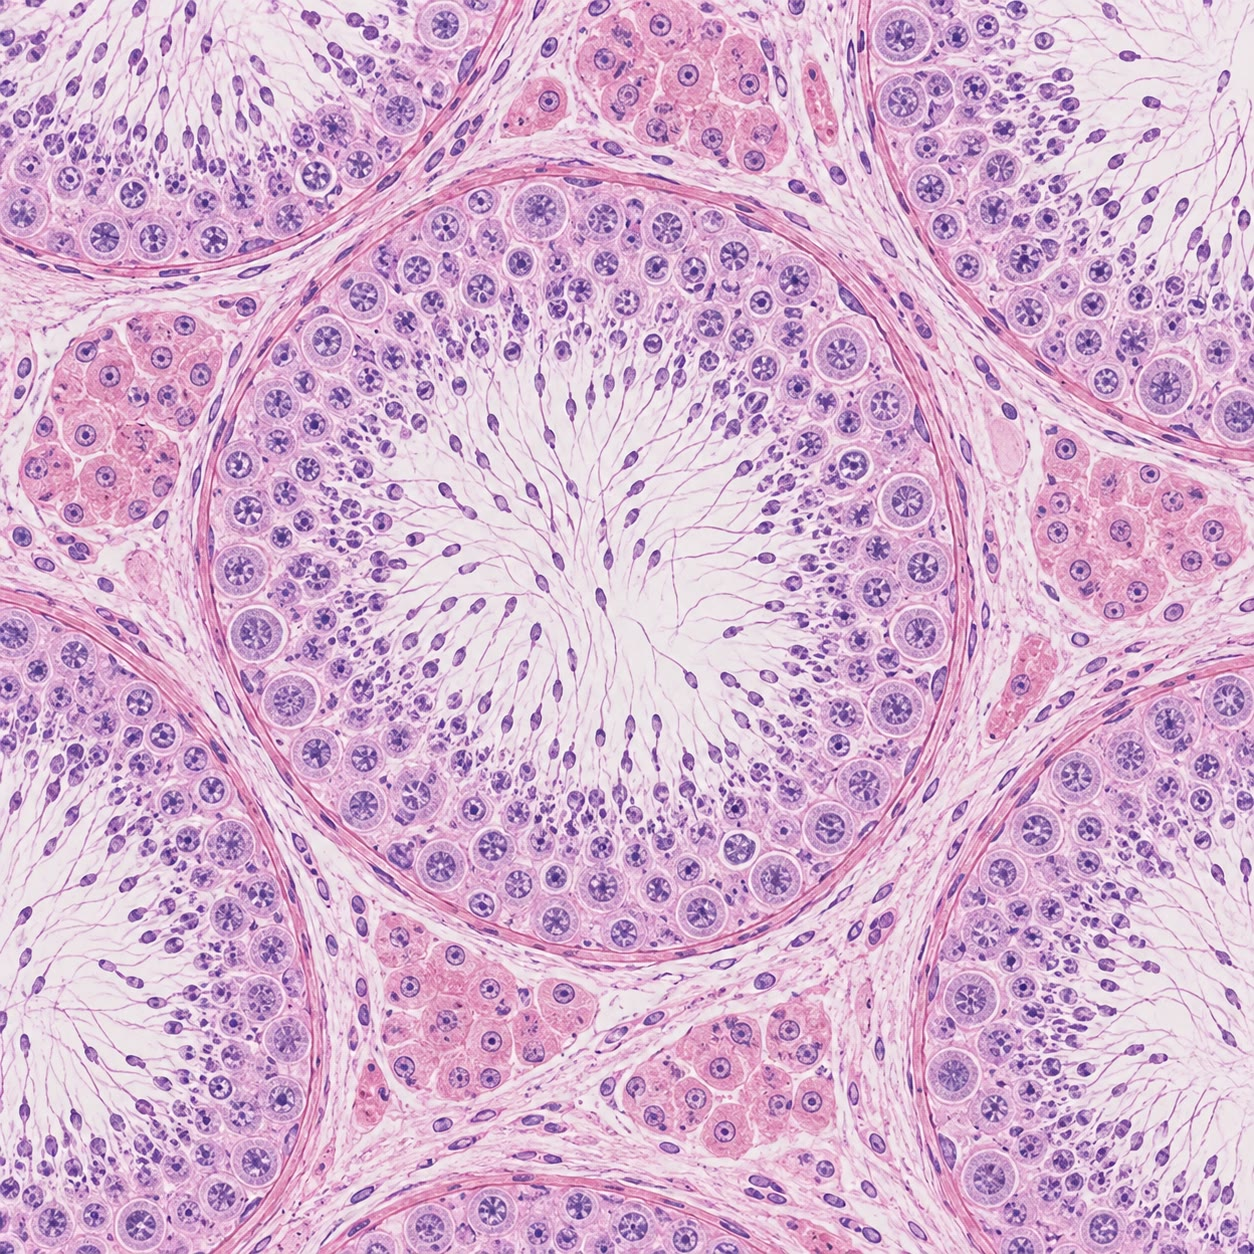
\includegraphics[width=0.42\linewidth]{images/book4/ai/b4-08-testis-histology.jpg}\hspace{0.04\linewidth}
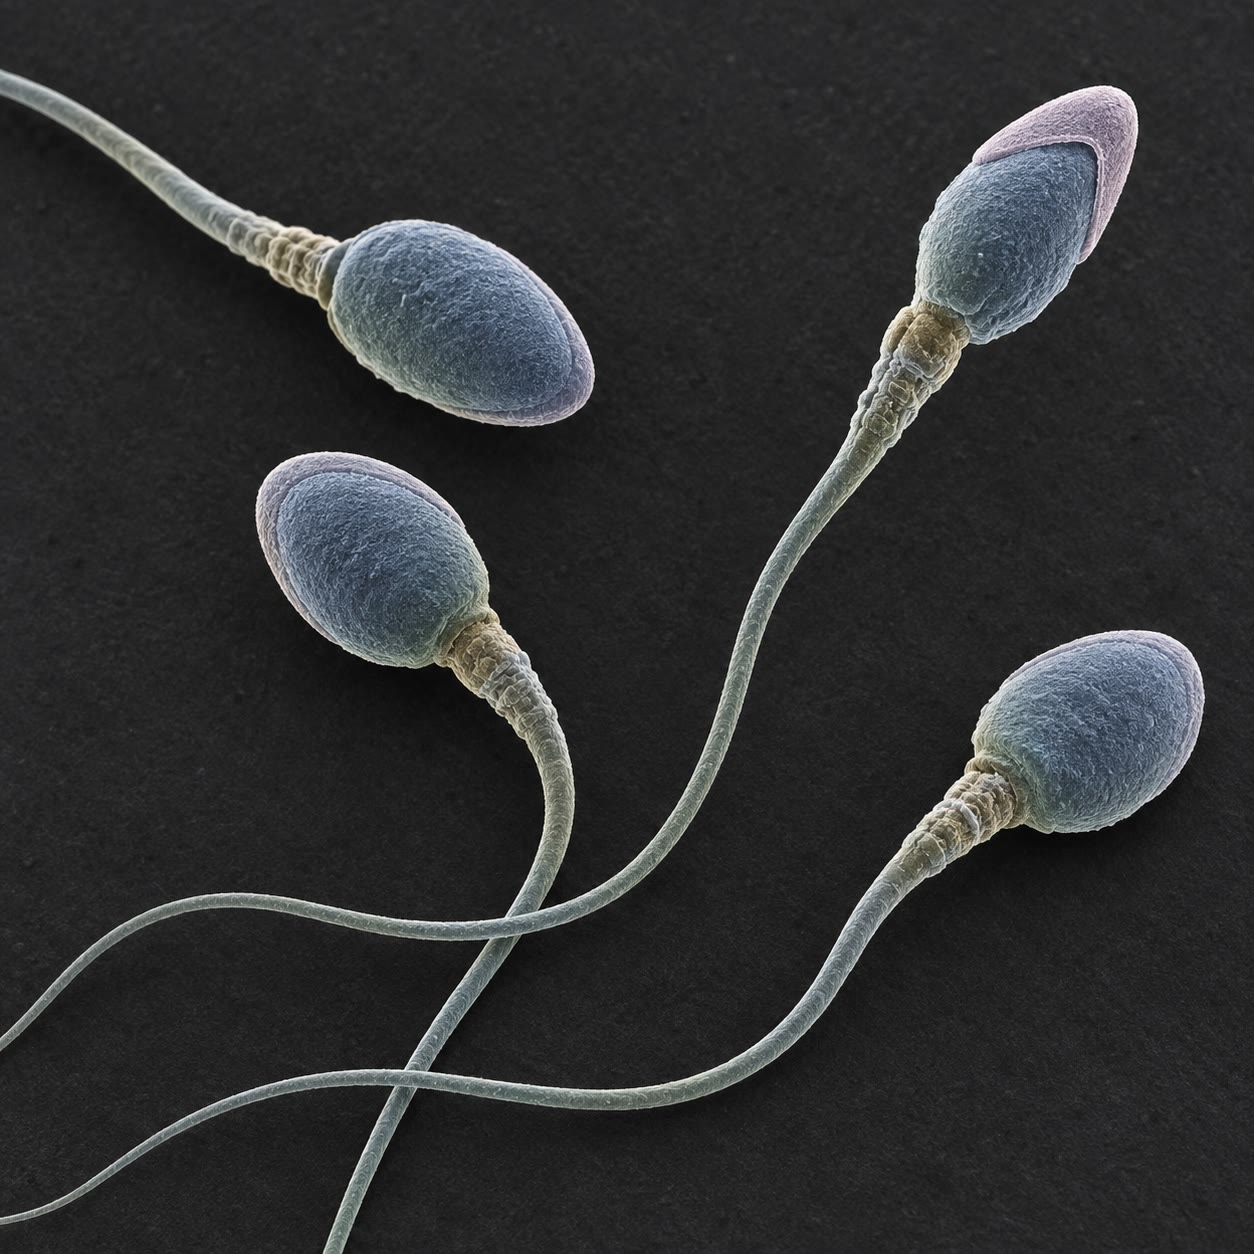
\includegraphics[width=0.42\linewidth]{images/book4/ai/b4-08-sperm-sem.jpg}

{\small على اليمين: نبيبات منوية في مقطع، والخلايا الإنتاشية مطبقة
من الجدار إلى اللمعة. وعلى اليسار: نطاف تحت المجهر الإلكتروني
الماسح، والغطاء القمي بادٍ على الرؤوس.}
\end{omfigure}

\begin{definition}[المبيض وتكوّن البويضات]\label{def:b2:mammal-reproduction:ovary}
\index{تكوّن البويضات}\index{جريب}\index{إباضة}\index{جسم أصفر}
تكوّن البويضات صورة مرآة \omterm{def:b2:mammal-reproduction:testis}{لتكوّن النطاف} في كل وجه تقريبًا. فالخلايا
\emph{المبيضية} لا تتكاثر إلا في الجنين: فعند الولادة تحمل
البنت مخزونًا من نحو مليون \emph{بويضة} أولية،
كل منها موقوفة في الطور التمهيدي الأول من \omterm{def:b2:meiosis-heredity:meiosis}{التقسم المنصّف} وملفوفة
بطبقة واحدة من الخلايا --- أي \emph{جريب بدئي} --- ولا تُصنع جديدة
أبدًا. ومن البلوغ، تنمو كل شهر مجموعة من الجريبات: فتكبر
البويضة، وتتكاثر خلايا \emph{الحُبيبية} المحيطة
طبقاتٍ، ويتكون \emph{قِراب} خارجي، وينفتح جوف مملوء بسائل
(وهو \emph{جريب غراف}، بقطر سنتيمترين)، ويبلغ واحد منها عادةً
\emph{الإباضة}: فتُقذف البويضة، وقد أتمت الآن \omterm{def:b2:meiosis-heredity:meiosis}{التقسم المنصّف} الأول
وتوقفت من جديد في الطور الاستوائي الثاني، مع هالتها من خلايا
الحُبيبية إلى قناة البيض. ويصير الجريب المفرَّغ
\emph{جسمًا أصفر}، وهو غدة مؤقتة للبروجستيرون. ويعطي \omterm{def:b2:meiosis-heredity:meiosis}{التقسم المنصّف}
بويضة واحدة وثلاثة أجسام قطبية ضئيلة --- إذ يذهب السيتوبلازم كله
إلى خلية واحدة --- ولا يكتمل \omterm{def:b2:meiosis-heredity:meiosis}{التقسم المنصّف} الثاني إلا إذا دخلت
نطفة. ومن المليون بويضة، تُباض نحو
\num{400} في العمر كله؛ وتنحل البقية
(\emph{الرتق})، وحين ينفد المخزون، نحو الخمسين،
تتوقف الدورات: وهو سن اليأس.
\end{definition}

\begin{omfigure}
\begin{tikzpicture}[every node/.style={font=\scriptsize}, >=stealth]
  % timeline of oogenesis vs spermatogenesis
  \draw[thick, ->] (0,3.0) -- (12.6,3.0); \node[anchor=west] at (12.6,3.0) {العمر};
  \foreach \x/\l in {0/{جنين}, 2.2/{ولادة}, 4.6/{بلوغ}, 10.2/{$\sim$50 سنة}}
    \draw (\x,3.1) -- (\x,2.9) node[above=0.15cm] {\l};
  % oogenesis line
  \node[anchor=east, omThm] at (-0.2,1.5) {تكوّن البويضات};
  \draw[very thick, omThm] (0,1.5) -- (1.6,1.5); \node[above, omThm, align=center] at (0.8,1.55) {الخلايا المبيضية\\تتكاثر};
  \draw[very thick, omThm, dashed] (1.6,1.5) -- (4.6,1.5); \node[below, omThm] at (3.1,1.45) {توقف في الطور التمهيدي الأول};
  \draw[very thick, omThm] (4.6,1.5) -- (10.2,1.5); \node[above, omThm, align=center] at (7.4,1.55) {إباضة واحدة في الشهر؛\\التقسم الأول يتم عند الإباضة، والثاني عند الإلقاح};
  \fill[omThm] (10.2,1.5) circle (0.07); \node[below, omThm] at (10.2,1.45) {نفاد المخزون};
  % spermatogenesis line
  \node[anchor=east, omDef] at (-0.2,0.3) {تكوّن النطاف};
  \draw[very thick, omDef, dashed] (0,0.3) -- (4.6,0.3); \node[above, omDef] at (2.3,0.35) {المنسليات ساكنة};
  \draw[very thick, omDef, ->] (4.6,0.3) -- (12.6,0.3); \node[above, omDef] at (8.6,0.35) {مستمر: $10^{8}$ نطفة في اليوم، 64 يومًا لكل منها، من خلايا جذعية};
\end{tikzpicture}

{\small تكوّنا الأعراس في الزمن. تُصنع البويضات كلها قبل الولادة
وتُطلق واحدة واحدة من مخزون منتهٍ؛ أما النطاف فتُصنع باستمرار من
خلايا جذعية طوال حياة البالغ.}
\end{omfigure}

\begin{omfigure}
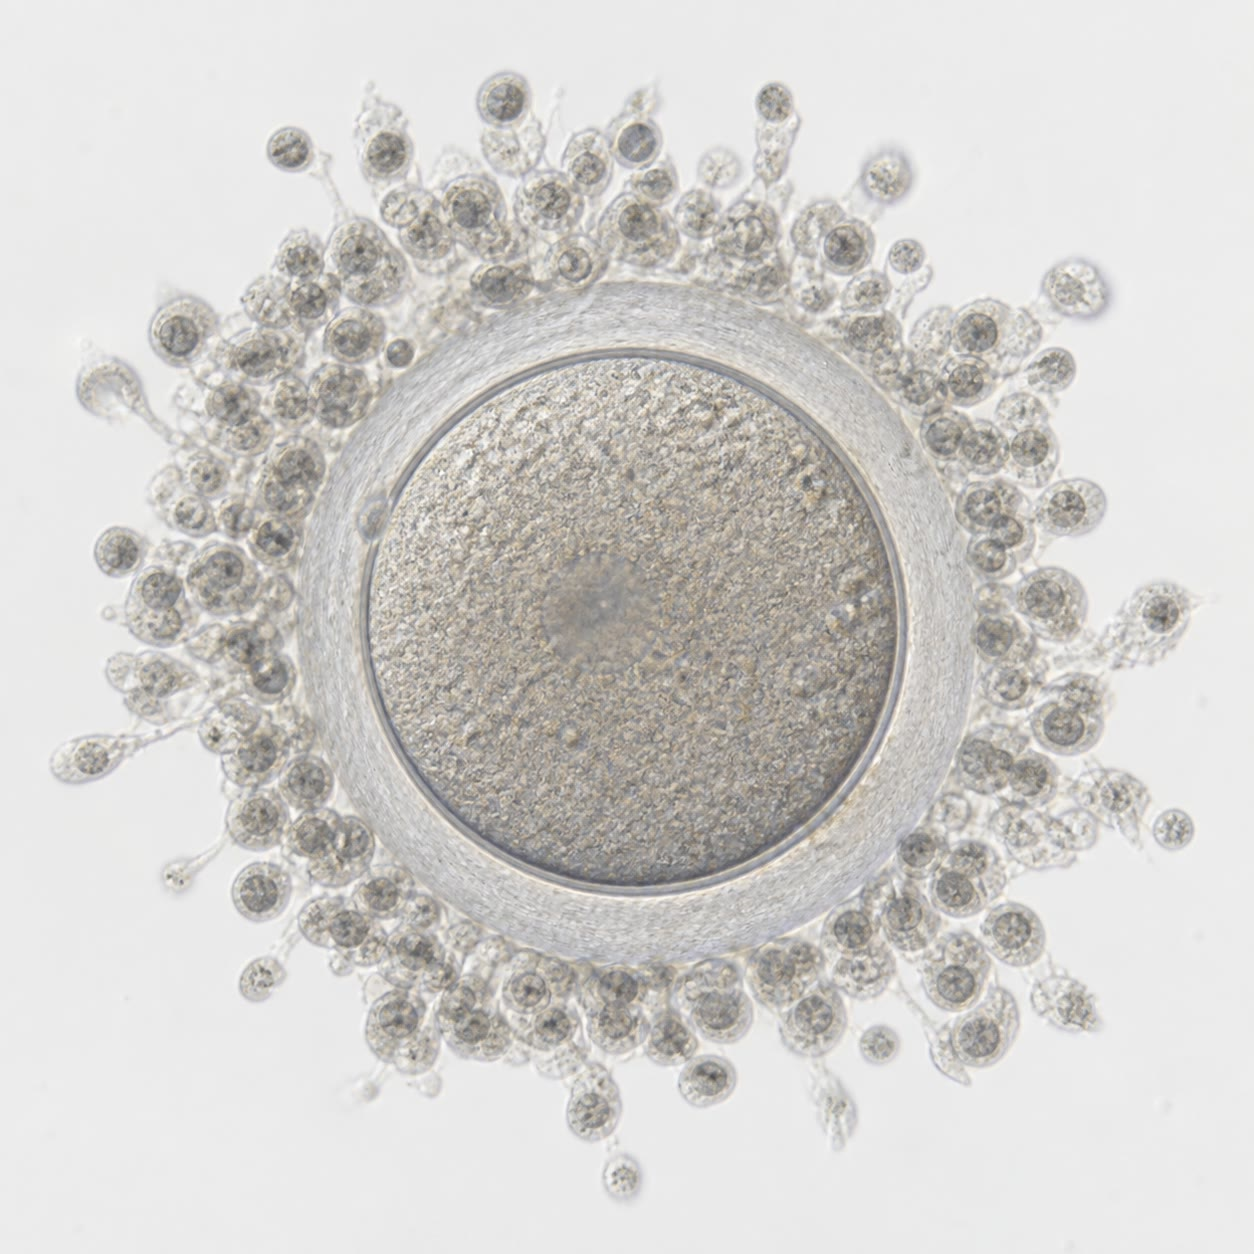
\includegraphics[width=0.46\linewidth]{images/book4/ai/b4-08-oocyte.jpg}

{\small بويضة مبيضة: الخلية، وغلافها الشفاف (\omterm{prop:b2:mammal-reproduction:fertilisation}{المنطقة
الشفافة})، وسحابة خلايا الحُبيبية التي غادرت \omterm{def:b2:mammal-reproduction:ovary}{الجريب} معها.}
\end{omfigure}

\section{الإلقاح}

\begin{proposition}[خطوات الإلقاح]\label{prop:b2:mammal-reproduction:fertilisation}
\index{إلقاح!عند الثدييات}\index{تفاعل الجسيم القمي}\index{المنطقة الشفافة}\index{تفاعل قشري}
النطاف الموضوعة في المهبل --- ونحوها $3\times 10^{8}$ --- تعبر
مخاط عنق الرحم، وتكنسها تقلصات الرحم صاعدةً، فتبلغ منها بضع مئات
أمبولة قناة البيض في غضون ساعة، حيث تنتظر
البويضة يومًا. وفي الطريق تمر النطاف
\emph{بالتأهيل}: فتجرّد إفرازات السبيل الأنثوي
أغشيتها من بروتينات الكساء وتجعلها مفرطة النشاط. وعند البويضة
تدفع نطفة طريقها بين خلايا الحُبيبية، وترتبط ببروتين سكري من
\emph{\omterm{prop:b2:mammal-reproduction:fertilisation}{المنطقة الشفافة}}، وتمر \emph{\omterm{prop:b2:mammal-reproduction:fertilisation}{بتفاعل الجسيم
القمي}}، فتطلق إنزيمات تهضم ممرًا عبر المنطقة؛
ويندمج غشاؤها بغشاء البويضة، فتدخل نواة النطفة. وتستجيب
البويضة في ثوانٍ: فيجتاحها الكالسيوم، وتطلق الحبيبات القشرية
إنزيمات تصلّب المنطقة وتجرّدها من مستقبلات النطاف
--- وهو \emph{\omterm{prop:b2:mammal-reproduction:fertilisation}{التفاعل القشري}}، أي الحاجز أمام \omterm{thm:b2:mammal-reproduction:poisson}{تعدد النطاف}.
وتتم البويضة \omterm{def:b2:meiosis-heredity:meiosis}{التقسم المنصّف} الثاني، وتطرح الجسم القطبي الثاني، ثم
تنسخ \emph{النواتان الأوليتان} الفرديتا الصيغة دناهما، وتلتقيان
وتدخلان أول تقسم خيطي: فتصير اللاقحة بعمر يوم. والنوعية
تكمن في بروتينات المنطقة، ولذلك لا تدخل نطفة فأر
بويضة بشرية.
\end{proposition}
\begin{proof}[شواهد]
لقّح إدواردز وستيبتو (1978) بويضة بشرية، مستخرجة
من المبيض قبيل \omterm{def:b2:mammal-reproduction:ovary}{الإباضة}، بنطاف مؤهَّلة في
طبق، ونمّيا الجنين إلى ثماني خلايا وأعاداه إلى
الرحم، فانغرس ووُلد: وهذا هو الإلقاح خارج الجسم.
وكانت كل خطوة من التسلسل أعلاه قد استُخرجت أولًا في
قنفذ البحر والفأر، حيث يمكن مراقبة الاندماج وموجة الكالسيوم
وإطلاق الحبيبات القشرية؛ وفي الفأر، يترك حذف أحد بروتيني
المنطقة السكريين (ZP2 أو ZP3) \omterm{def:b2:genome-diversification:mutation}{بالطفرة} بويضات لا تستطيع النطاف
الارتباط بها.
\end{proof}

\begin{theorem}[لماذا تحتاج بويضة واحدة إلى ملايين النطاف]\label{thm:b2:mammal-reproduction:poisson}
\index{تعدد النطاف}
إذا بلغت كل نطفة من $N$ نطفة موضوعة سطحَ البويضة
مستقلةً باحتمال صغير $\pi$، كان عدد الواصلات
بواسونيًا متوسطه $m = N\pi$، وكان احتمال وصول واحدة على الأقل
\[
P = 1 - e^{-m}.
\]
فمع $N = 3\times 10^{8}$ و$\pi \approx 10^{-8}$ يكون $m \approx 3$
و$P \approx 0.95$؛ ومع $N = 2\times 10^{7}$ (وهي العتبة
السريرية لقلة النطاف) يكون $m = 0.2$ و$P = 0.18$. والحساب نفسه
يبين لماذا كان الحاجز أمام \omterm{thm:b2:mammal-reproduction:poisson}{تعدد النطاف} لا غنى عنه: فحين يكون
$P$ عاليًا تصل عدة نطاف خلال ثوانٍ بعضها من بعض،
والبويضة التي تدخلها نطفتان تكون ثلاثية الصيغة وتموت.
\end{theorem}
\begin{proof}
كل نطفة تجربة مستقلة باحتمال نجاح $\pi$؛
وعدد النجاحات ثنائي الحد، وهو من أجل $N$ الكبيرة و$\pi$
الصغيرة بواسوني بمتوسط $N\pi$. واحتمال صفر
نجاح هو $e^{-m}$، فيكون احتمال واحد على الأقل $1 - e^{-m}$؛
واحتمال اثنتين أو أكثر هو $1 - e^{-m}(1 + m)$، أي نحو $0.8$ من أجل
$m = 3$.
\end{proof}

\begin{omfigure}
\begin{tikzpicture}[every node/.style={font=\scriptsize}, >=stealth]
  \foreach \x/\lab in {0/{1. النطفة ترتبط\\بالمنطقة الشفافة}, 3.3/{2. تفاعل الجسيم القمي:\\إنزيمات تشق طريقًا}, 6.6/{3. اندماج الغشاءين؛\\وموجة كالسيوم}, 9.9/{4. التفاعل القشري:\\تصلّب المنطقة الشفافة،\\وإتمام التقسم المنصّف II}} {
    \begin{scope}[xshift=\x cm]
      \draw[thick, fill=omThm!8] (0,0) circle (0.9);
      \draw[thick, omExo!70!black] (0,0) circle (1.15);
      \node[below, align=center] at (0,-1.3) {\lab};
    \end{scope}
  }
  % stage 1: sperm at zona
  \draw[thick, fill=omDef!50] (-1.45,0.1) ellipse (0.18 and 0.11); \draw[thick, omDef] (-1.63,0.1) .. controls (-2.0,0.4) and (-2.2,-0.2) .. (-2.5,0.1);
  % stage 2: sperm digging through zona
  \begin{scope}[xshift=3.3cm]
    \fill[white] (-1.2,0.0) circle (0.12);
    \draw[thick, fill=omDef!50] (-1.05,0.05) ellipse (0.18 and 0.11); \draw[thick, omDef] (-1.23,0.05) .. controls (-1.6,0.35) and (-1.8,-0.25) .. (-2.1,0.05);
    \foreach \a in {150,170,190,210} \draw[omProp, thick] (-1.2,0.0) -- ++(\a:0.25);
  \end{scope}
  % stage 3: fused, calcium wave
  \begin{scope}[xshift=6.6cm]
    \fill[white] (-1.15,0.0) circle (0.12);
    \draw[thick, fill=omDef!50] (-0.75,0.0) ellipse (0.18 and 0.11);
    \draw[thick, omDef] (-0.93,0.0) .. controls (-1.3,0.3) and (-1.5,-0.3) .. (-1.8,0.0);
    \foreach \r in {0.35,0.55,0.75} \draw[omProp, thick] (-0.75,0) ++(-60:\r) arc (-60:60:\r);
  \end{scope}
  % stage 4: hardened zona, polar body, pronuclei
  \begin{scope}[xshift=9.9cm]
    \draw[very thick, omExo!70!black] (0,0) circle (1.15);
    \draw[thick, fill=omDef!30] (-0.25,0.05) circle (0.2); \draw[thick, fill=omThm!30] (0.25,0.05) circle (0.2);
    \draw[thick, fill=omThm!20] (0.55,0.95) circle (0.12);
    \node[anchor=west] at (1.2,0.9) {جسم قطبي};
    \draw (0.45,0.05) -- (1.2,-0.35); \node[anchor=west] at (1.2,-0.35) {نواتان أوليتان};
  \end{scope}
\end{tikzpicture}

{\small الإلقاح في أربع خطوات: الارتباط \omterm{prop:b2:mammal-reproduction:fertilisation}{بالمنطقة الشفافة}، \omterm{prop:b2:mammal-reproduction:fertilisation}{وتفاعل
الجسيم القمي}، والاندماج وموجة الكالسيوم، \omterm{prop:b2:mammal-reproduction:fertilisation}{والتفاعل القشري} الذي يغلق
البويضة أمام سائر النطاف بينما تتم
\omterm{def:b2:meiosis-heredity:meiosis}{التقسم المنصّف}.}
\end{omfigure}

\section{الانغراس والمشيمة}

\begin{definition}[التفلج والكيسة الأريمية والانغراس]\label{def:b2:mammal-reproduction:implantation}
\index{كيسة أريمية}\index{أرومة مغذية}\index{كتلة خلوية داخلية}\index{انغراس}
تنقسم اللاقحة كل اثنتي عشرة إلى عشرين ساعة دون أن تنمو
(\emph{التفلج}) وهي تُنقل نزولًا في قناة البيض: خليتان، فأربع،
فثمان، فكرة متراصة من ست عشرة (\emph{التوتية})، وفي اليوم الخامس
\emph{كيسة أريمية} من نحو مئة خلية: طبقة خارجية هي
\emph{الأرومة المغذية}، حول جوف، مع كتلة خلايا في جانب،
هي \emph{الكتلة الخلوية الداخلية}. والأرومة المغذية ستبني
\omterm{def:b2:mammal-reproduction:placenta}{المشيمة} والأغشية؛ والكتلة الخلوية الداخلية ستصير الجنين
--- وتعطي، إذا أُخرجت في هذا الطور، خلايا جذعية جنينية. وفي اليوم
السادس تفقس الكيسة الأريمية من منطقتها الشفافة، وتلتصق ببطانة
الرحم، وتغزوها الأرومة المغذية: إذ تندمج الخلايا في جبهة
عديدة النوى تهضم النسيج الأمومي وتفتح الشعيرات الأمومية،
حتى يصير الجنين في اليوم الثاني عشر مدفونًا في الجدار
مغمورًا في الدم الأمومي. وهذا هو \emph{الانغراس}. وهو
لا ينجح إلا في رحم هيأه البروجستيرون، في نافذة من
أيام قليلة؛ ونحو نصف الحمول البشرية يفشل قبل هذه الخطوة أو عندها،
من أخطاء صبغية في البويضة عادةً.
\end{definition}

\begin{omfigure}
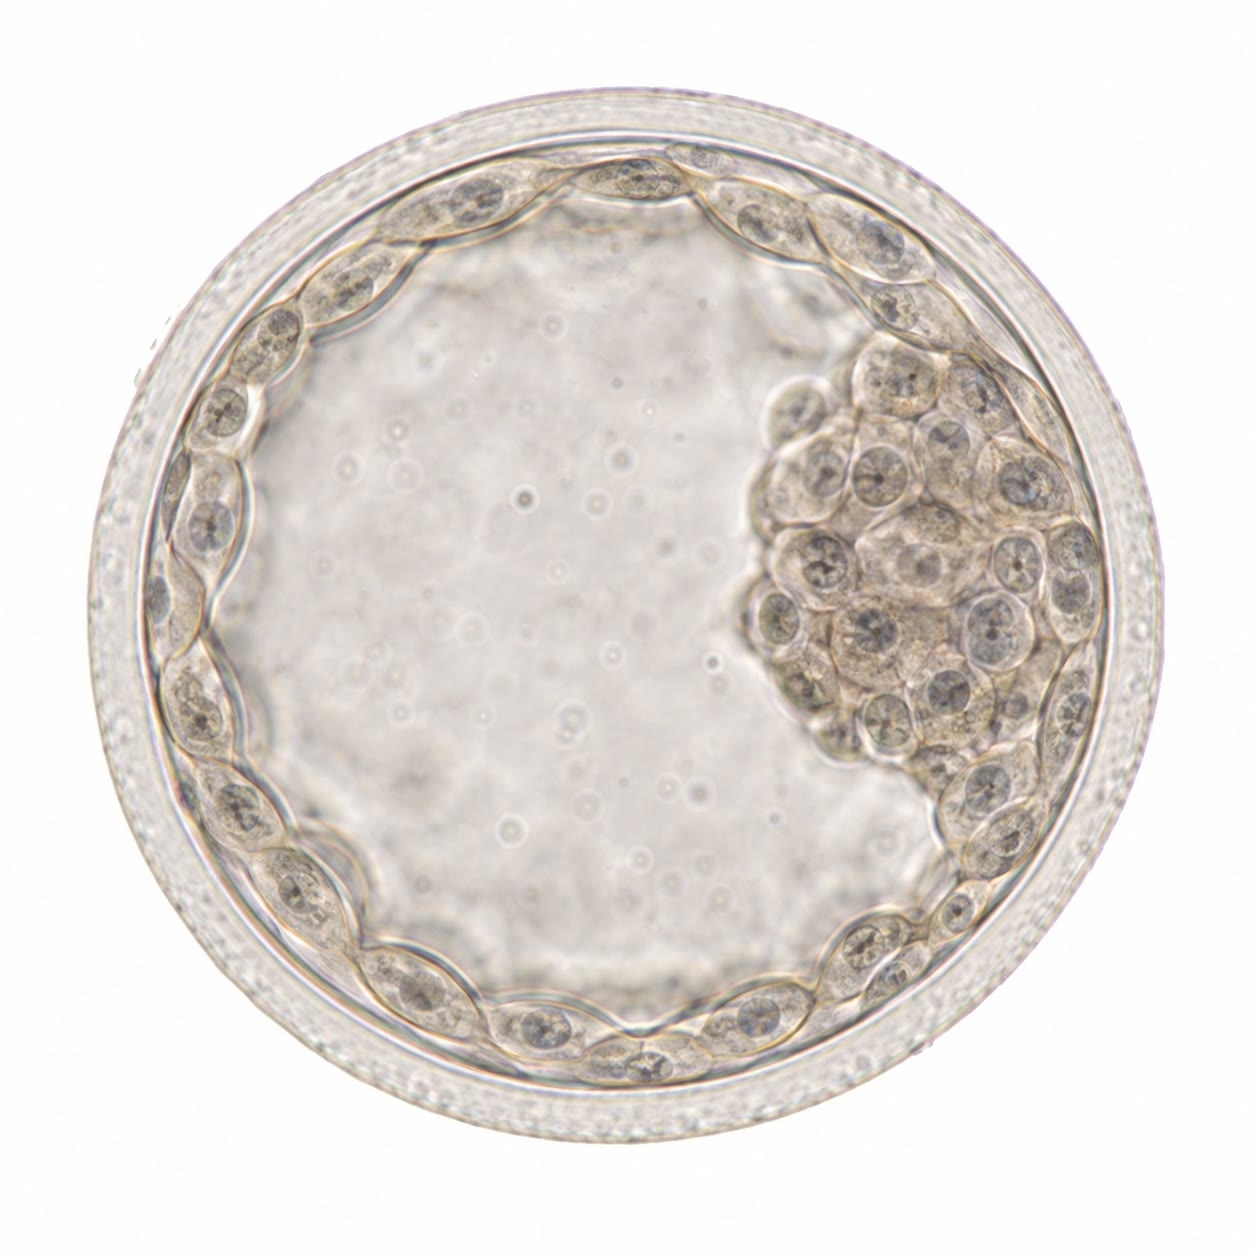
\includegraphics[width=0.42\linewidth]{images/book4/ai/b4-08-blastocyst.jpg}

{\small \omterm{def:b2:mammal-reproduction:implantation}{كيسة أريمية} في اليوم الخامس: \omterm{def:b2:mammal-reproduction:implantation}{الأرومة المغذية} الخارجية حول
الجوف، \omterm{def:b2:mammal-reproduction:implantation}{والكتلة الخلوية الداخلية} --- أي الجنين المقبل --- في
جانب.}
\end{omfigure}

\begin{definition}[المشيمة]\label{def:b2:mammal-reproduction:placenta}
\index{مشيمة}\index{زغابة مشيمائية}\index{حبل سري}
\emph{المشيمة} عضو يصنعه الجنين (المشيماء، من \omterm{def:b2:mammal-reproduction:implantation}{الأرومة
المغذية}) والأم (بطانة الرحم) معًا.
وتتدلى \emph{زغابات مشيمائية} إصبعية، متفرعة إلى سطح نحو
\qty{12}{m^2} عند الولادة، في بحيرات من دم أمومي تسلّمه
شرايين الرحم بنصف لتر في الدقيقة؛ وداخل كل زغابة
تجري شعيرات جنينية، موصولة بالجنين عبر شريانين
ووريد واحد في \emph{الحبل السري}. والدمان لا يختلطان قط:
فيفصلهما جدار الزغابة، وهو بضعة ميكرومترات من
\omterm{def:b2:mammal-reproduction:implantation}{الأرومة المغذية} وبطانة الشعيرة، ينتشر عبرها الأكسجين
و$\mathrm{CO_2}$ والماء والبولة والجزيئات المنحلّة في الدهن،
ويُنقل الغلوكوز والحموض الأمينية بناقلات،
وتُعبَّر الأضداد الأمومية (IgG) بمستقبل، فتعطي المولود
أشهره الأولى من المناعة. والمشيمة غدة أيضًا: فمن
الأيام الأولى تفرز \omterm{def:b2:mammal-reproduction:implantation}{الأرومة المغذية} \emph{موجهة الغدد
التناسلية المشيمائية البشرية} (hCG)، وهي تبقي \omterm{def:b2:mammal-reproduction:ovary}{الجسم الأصفر} يصنع
البروجستيرون، ومن الشهر الثالث تصنع المشيمة نفسها
البروجستيرون والإستروجينات التي تصون الحمل
(\cref{ch:b2:reproductive-hormones}). فهي، في الواقع، رئة
ومعي وكلية وغدة صماء تنمو تسعة أشهر
وتُطرح عند الولادة.
\end{definition}

\begin{omfigure}
\begin{tikzpicture}[every node/.style={font=\scriptsize}, >=stealth]
  % maternal blood space
  \fill[omThm!12] (0,0) rectangle (8,3.6);
  \node[omThm!80!black, align=center] at (1.1,2.6) {دم أمومي\\(الفراغ بين\\الزغابات)};
  % uterine wall at bottom
  \fill[omExo!30] (0,-0.6) rectangle (8,0); \node at (4,-0.3) {جدار الرحم (أمومي)};
  \draw[->, thick, omThm] (1.0,-0.6) -- (1.0,0.6); \node[omThm, anchor=west] at (1.05,0.3) {شريان حلزوني};
  \draw[->, thick, omDef!60!black] (7.0,0.6) -- (7.0,-0.6); \node[omDef!60!black, anchor=east] at (6.95,0.3) {وريد رحمي};
  % chorionic plate at top
  \fill[omDef!20] (0,3.6) rectangle (8,4.4); \node at (4,4.0) {الصفيحة المشيمائية (جنينية)};
  % villi hanging down
  \foreach \x in {2.6,4.2,5.8} {
    \draw[thick, fill=omDef!8] (\x-0.35,3.6) -- (\x-0.4,1.4) .. controls (\x-0.4,0.9) and (\x+0.4,0.9) .. (\x+0.4,1.4) -- (\x+0.35,3.6);
    \draw[thick, omThm!70!black] (\x-0.15,3.6) -- (\x-0.15,1.5) .. controls (\x-0.15,1.25) and (\x+0.15,1.25) .. (\x+0.15,1.5) -- (\x+0.15,3.6);
    \foreach \y in {2.0,2.7} { \draw[thick, fill=omDef!8] (\x-0.4,\y) .. controls (\x-0.9,\y+0.1) and (\x-0.9,\y-0.4) .. (\x-0.4,\y-0.3); }
  }
  % umbilical vessels
  \draw[very thick, omThm!70!black] (4.2,4.4) -- (4.2,5.0) node[above, align=center] {الوريد السري (إلى الجنين)\\والشريانان};
  \draw[very thick, omDef!60!black] (3.9,4.4) -- (3.9,5.0); \draw[very thick, omDef!60!black] (4.5,4.4) -- (4.5,5.0);
  % exchange arrows
  \draw[<->, thick] (3.0,2.2) -- (3.75,2.2); \node[anchor=west, align=left] at (8.3,1.5) {عبر الجدار: \textcolor{omThm}{O$_2$، والغلوكوز،}\\\textcolor{omThm}{والحموض الأمينية، وIgG} إلى الجنين؛\\\textcolor{omDef!60!black}{وCO$_2$، والبولة} إلى الأم};
  \node[anchor=west, align=left] at (8.3,3.0) {جدار الزغابة: أرومة مغذية\\+ بطانة شعيرة جنينية،\\بضعة ميكرومترات};
  \draw (6.2,2.5) -- (8.3,3.0);
\end{tikzpicture}

{\small \omterm{def:b2:mammal-reproduction:placenta}{المشيمة}: تتدلى زغابات جنينية، تحمل شعيرات جنينية، في
فراغ مملوء بدم أمومي من الشرايين الحلزونية. ويتبادل الدمان عبر
جدار الزغابة ولا يختلطان أبدًا.}
\end{omfigure}

\begin{theorem}[التبادل عبر المشيمة]\label{thm:b2:mammal-reproduction:fick}
\index{قانون فيك!المشيمة}
الغاز العابر غشاءً مساحته $A$ وثخنه $d$ ينتقل بمعدل
$J = K\,A\,\Delta P/d$، حيث $\Delta P$ فرق
ضغطه الجزئي و$K$ نفوذية النسيج. وللأكسجين
في النسيج $K \approx \qty{3e-8}{mL/(cm.min.mmHg)}$؛ فمع $A =
\qty{12}{m^2}$، و$d = \qty{3.5}{\micro m}$، و$\Delta P =
\qty{20}{mmHg}$ (أي \qty{40}{mmHg} أموميًا في الفراغ بين الزغابات
في مقابل \qty{20}{mmHg} في الشريان السري)، تستطيع \omterm{def:b2:mammal-reproduction:placenta}{المشيمة}
تمرير نحو \qty{200}{mL} من الأكسجين في الدقيقة، أي نحو ثمانية أضعاف
\qty{25}{mL/min} التي يستهلكها جنين تام. فنقل الأكسجين إذن
لا يحده الانتشار بل الجريان الدموي؛ والجنين يعمل عند ضغط
أكسجين منخفض ويعوّض بهيموغلوبين أعلى ألفة
وبعدد كريات حمر أكبر.
\end{theorem}
\begin{proof}
ينص قانون فيك على أن التدفق يتناسب مع التدرج
$\Delta P/d$ ومع المساحة؛ والثابت $K$ يستوعب انحلالية
الغاز في النسيج ومعامل انتشاره فيه. وعدديًا:
$3\times 10^{-8}\times 1.2\times 10^{5}\times 20/(3.5\times 10^{-4})
= \qty{206}{mL/min}$ مع $A$ بوحدة \unit{cm^2} و$d$ بوحدة \unit{cm}.
والطلب الجنيني نحو \qty{7}{mL} لكل كيلوغرام في الدقيقة من أجل
\qty{3.5}{kg}.
\end{proof}

\section{الحمل والولادة والإرضاع}

\begin{proposition}[الحمل والولادة]\label{prop:b2:mammal-reproduction:birth}
\index{حمل}\index{مخاض}\index{أوكسيتوسين}
يدوم الحمل \num{20} يومًا عند الفأر، و\num{280} عند الإنسان، و\num{660}
عند الفيل --- أي تقريبًا كجذر كتلة الجسم الرابع، مع بطء
الرئيسيات بالقياس إلى قياسها. ويصونه البروجستيرون،
الذي يبقي عضلة الرحم هادئة وعنقه مغلقًا. والولادة
(\emph{المخاض}) يطلقها الجنين نفسه: فكورتيزول كظره،
المرتفع عند التمام، ينقل \omterm{def:b2:mammal-reproduction:placenta}{المشيمة} من البروجستيرون إلى
الإستروجين، الذي يزوّد الرحم بمستقبلات الأوكسيتوسين
ووصلات فجوية ويبدأ إطلاق البروستاغلاندينات. ثم تتولى
\emph{تغذية راجعة موجبة} الأمر: فيضغط الرأس على عنق الرحم، وتشير
الأعصاب الحسية إلى الوطاء، ويُطلق \emph{الأوكسيتوسين} من
النخامى الخلفية، فينقبض الرحم، فيضغط الرأس أشد؛
وتتصاعد الحلقة حتى الولادة، وعندها ينتهي المنبه
وتتوقف الحلقة --- وهي من التغذيات الراجعة الموجبة القليلة في
الفيزيولوجيا، ومن تلك التي لا بد أن تنتهي بحدث. وتُطرح \omterm{def:b2:mammal-reproduction:placenta}{المشيمة}
بعد دقائق.
\end{proposition}
\begin{proof}[شواهد]
بيّن فيرغسون (1941) في الأرنب أن توسيع عنق الرحم
يستثير تقلصات رحمية وأن قطع النخاع الشوكي أو
نزع النخامى الخلفية يلغي الاستجابة: أي إنه
منعكس عصبي صماوي من عنق الرحم إلى النخامى إلى الرحم. أما
الأوكسيتوسين، الذي عزله واصطنعه دو فينيو سنة 1953، فهو اليوم الدواء
المعياري لتحريض المخاض.
\end{proof}

\begin{proposition}[الإرضاع]\label{prop:b2:mammal-reproduction:lactation}
\index{إرضاع}\index{برولاكتين}\index{حليب}
الغدة الثديية، وهي غدة عرقية معدّلة، تُبنى خلال الحمل
بالإستروجين والبروجستيرون والبرولاكتين لكن البروجستيرون يمنعها من
الإفراز؛ فحين تغادر \omterm{def:b2:mammal-reproduction:placenta}{المشيمة}، يهبط البروجستيرون، وتبدأ
الأسناخ، تحت \emph{البرولاكتين} من النخامى الأمامية،
بصنع الحليب. ويدير العمليةَ منعكسان: فالرضاعة
تنبه إطلاق البرولاكتين (الذي يصون الاصطناع
ويكبت \omterm{def:b2:mammal-reproduction:ovary}{الإباضة}) وإطلاق الأوكسيتوسين (الذي يقبض
الخلايا حول الأسناخ فيقذف الحليب). ويحمل حليب الإنسان
نحو \qty{7}{\%} لاكتوزًا، و\qty{4}{\%} دهنًا، و\qty{1}{\%} بروتينًا،
و\qty{2.9}{kJ/mL}؛ و\emph{اللبأ} في الأيام الأولى غني
بالأضداد (IgA) التي تكسو معي الرضيع. وتصنع الأم نحو
\qty{750}{mL} في اليوم، بكلفة نحو \qty{2.5}{MJ} --- أي ربع
طعامها --- أشهرًا؛ فالإرضاع أغلى أجزاء التكاثر
عند الثدييات وهو الذي سمّى الصف.
\end{proposition}

\section{صنع الجنسين}

\begin{proposition}[تحديد الجنس وتمايزه]\label{prop:b2:mammal-reproduction:sex}
\index{SRY}\index{الهرمون المضاد لمولر}\index{تمايز جنسي}
حتى الأسبوع السادس يكون للجنين البشري من أي جنس العتاد
نفسه: منسل غير متمايز، وزوجا قنوات (\emph{ولفية}
و\emph{مولرية}) وأعضاء تناسلية خارجية محايدة. والمورّثة
\emph{SRY} على الصبغي Y تشتعل في المنسل فتحوله
إلى خصية؛ ودونها يصير المنسل مبيضًا. ثم تفعل \omterm{def:b2:mammal-reproduction:testis}{الخصية}
الجنينية أمرين: فتفرز خلايا سرتولي فيها
\emph{\omterm{prop:b2:mammal-reproduction:sex}{الهرمون المضاد لمولر}}، الذي يجعل القنوات المولرية
تضمر، وتفرز خلايا لايديغ فيها \emph{التستوستيرون}، الذي
يبقي القنوات الولفية (وهي البربخ والأسهر
والحويصلان المنويان المقبلة) و، محوَّلًا إلى ديهدروتستوستيرون، يشكّل
الأعضاء التناسلية الخارجية قضيبًا وصفنًا. وفي غياب
الإشارتين تضمر القنوات الولفية، وتصير القنوات المولرية
قنوات البيض والرحم وأعلى المهبل، وتنمو الأعضاء التناسلية
أنثوية. فالمسلك الأنثوي هو المسلك المسلوك حين لا يُقال شيء:
أما المسلك الذكري فلا بد أن تفرضه \omterm{def:b2:mammal-reproduction:testis}{الخصية} فرضًا، وكل خطوة
يفشل فيها الفرض --- مورّثة SRY طافرة، أو مستقبل هرموني
مفقود --- تعطي فردًا XY بجسم أنثوي أو وسطي.
\end{proposition}
\begin{proof}[شواهد]
نزع جوست (1947) مناسل أجنة أرانب في الرحم
قبل أن تتمايز قنواتها: فنمت للأجنة المخصية من أي جنس
صبغي رحمٌ وقناتا بيض وأعضاء تناسلية
أنثوية. وبلورة تستوستيرون مغروسة في جنين مخصي
أبقت القنوات الولفية في ذلك الجانب لكنها لم تُزل
القنوات المولرية؛ أما خصية جنينية مطعّمة ففعلت الأمرين، في جانبها:
فلا بد أن تصنع \omterm{def:b2:mammal-reproduction:testis}{الخصية} عاملًا ثانيًا، مجهولًا حينها، يكبت
القنوات الأنثوية، عُرف بعد ثلاثين سنة \omterm{prop:b2:mammal-reproduction:sex}{بالهرمون المضاد
لمولر}. ثم عيّن الأثر العاكس للجنس لقطعة صغيرة من الصبغي Y
موضع المفتاح في \emph{SRY} (1990)، ونما فأر جُعل
XX بمورّثة \emph{Sry} وحدها ذكرًا.
\end{proof}

\begin{omfigure}
\begin{tikzpicture}[every node/.style={font=\scriptsize}, >=stealth]
  \node[draw, rounded corners, fill=omExo!25, align=center] (g) at (0,0) {منسل غير متمايز\\جملتا قنوات};
  \node[draw, rounded corners, fill=omDef!15, align=center] (t) at (4.2,1.4) {خصية\\(\emph{SRY} حاضرة)};
  \node[draw, rounded corners, fill=omThm!15, align=center] (o) at (4.2,-1.4) {مبيض\\(لا \emph{SRY})};
  \node[draw, rounded corners, fill=omDef!15, align=center] (amh) at (8.6,2.3) {AMH: القنوات المولرية تضمر};
  \node[draw, rounded corners, fill=omDef!15, align=center] (tst) at (8.6,0.6) {التستوستيرون: القنوات الولفية تبقى؛\\وDHT: أعضاء تناسلية ذكرية};
  \node[draw, rounded corners, fill=omThm!15, align=center] (f) at (8.6,-1.4) {لا إشارة: القنوات الولفية تضمر،\\والمولرية $\to$ قنوات بيض ورحم؛\\وأعضاء تناسلية أنثوية};
  \draw[->, thick] (g) -- (t); \draw[->, thick] (g) -- (o);
  \draw[->, thick] (t) -- (amh); \draw[->, thick] (t) -- (tst); \draw[->, thick] (o) -- (f);
\end{tikzpicture}

{\small \omterm{prop:b2:mammal-reproduction:sex}{التمايز الجنسي}: \omterm{def:b2:mammal-reproduction:testis}{الخصية}، التي تصنعها \emph{SRY}،
تفرض المسلك الذكري بهرمونين؛ وفي غيابهما ينمو الجسم
أنثويًا.}
\end{omfigure}

\section{تمارين}

\begin{exercise}[$\star$]\label{exo:b2:mammal-reproduction:1}
قارن \omterm{def:b2:mammal-reproduction:testis}{تكوّن النطاف} \omterm{def:b2:mammal-reproduction:ovary}{بتكوّن البويضات}: متى تنقسم الخلايا الجذعية،
وكم عروسًا يعطي \omterm{def:b2:meiosis-heredity:meiosis}{التقسم المنصّف} الواحد، وكم يستغرق صنع عروس،
وأين تقع التوقفات، وكم عروسًا يُنتَج في العمر
كله.
\end{exercise}

\begin{exercise}[$\star$]\label{exo:b2:mammal-reproduction:2}
اذكر خطوات الإلقاح من وصول نطفة إلى \omterm{prop:b2:mammal-reproduction:fertilisation}{المنطقة الشفافة} حتى أول تقسم
خيطي، وقل أي خطوة تسد الطريق أمام \omterm{thm:b2:mammal-reproduction:poisson}{تعدد النطاف}.
\end{exercise}

\begin{exercise}[$\star$]\label{exo:b2:mammal-reproduction:3}
سمِّ جمهرتي خلايا \omterm{def:b2:mammal-reproduction:implantation}{الكيسة الأريمية} ومصير كل منهما. وفي أي يوم يبدأ
\omterm{def:b2:mammal-reproduction:implantation}{الانغراس}، وأي هرمون يجب أن يكون قد هيأ الرحم؟
\end{exercise}

\begin{exercise}[$\star$]\label{exo:b2:mammal-reproduction:4}
قل في كل مما يأتي هل يعبر \omterm{def:b2:mammal-reproduction:placenta}{المشيمة} وكيف: الأكسجين، والغلوكوز،
والكريات الحمر الأمومية، والأضداد IgG، والبولة،
والكحول، ومعظم البكتيريا.
\end{exercise}

\begin{exercise}[$\star\star$]\label{exo:b2:mammal-reproduction:5}
مع $\pi = 10^{-8}$ للنطفة الواحدة، احسب احتمال
الإلقاح من أجل أعداد نطاف $3\times 10^{8}$ و$10^{8}$
و$4\times 10^{7}$ و$10^{7}$. وعند أي عدد يهبط دون
النصف؟ وماذا يقول هذا عن شكل منحني الجرعة--الاستجابة
للخصوبة بدلالة عدد النطاف؟
\end{exercise}

\begin{exercise}[$\star\star$]\label{exo:b2:mammal-reproduction:6}
تولد بنت ولها $10^{6}$ بويضة، ويصير لها \num{300000} عند البلوغ
(في سن 13) ونحو \num{1000} في سن 50، وقد أباضت \num{400}.
احسب متوسط معدل الرتق (البويضات المفقودة في اليوم) قبل البلوغ
وبعده، وقارنه بمعدل \omterm{def:b2:mammal-reproduction:ovary}{الإباضة}.
\end{exercise}

\begin{exercise}[$\star\star$]\label{exo:b2:mammal-reproduction:7}
للهيموغلوبين الجنيني ضغط نصف إشباع $P_{50} =
\qty{19}{mmHg}$، وللبالغ \qty{27}{mmHg}؛ وخذ
الإشباع $S = P^{n}/(P_{50}^{n} + P^{n})$ مع $n = 2.7$.
احسب الإشباعين عند \qty{30}{mmHg}، وهو الضغط في الوريد
السري، واشرح الميزة.
\end{exercise}

\begin{exercise}[$\star\star$]\label{exo:b2:mammal-reproduction:8}
يظهر hCG في الدم الأمومي عند \omterm{def:b2:mammal-reproduction:implantation}{الانغراس} (اليوم 7 بعد
الإلقاح) عند نحو \qty{1}{IU/L} ويتضاعف كل يومين؛ ويكشف
اختبار الحمل \qty{25}{IU/L}. ففي أي يوم بعد
الإلقاح يصير الاختبار موجبًا؟ وفي أي يوم بعد آخر
دورة طمثية (\omterm{def:b2:mammal-reproduction:ovary}{والإباضة} في اليوم 14)؟
\end{exercise}

\begin{exercise}[$\star\star$]\label{exo:b2:mammal-reproduction:9}
أعد حساب نقل الأكسجين المشيمي في المبرهنة من أجل
\omterm{def:b2:mammal-reproduction:placenta}{مشيمة} مساحتها \qty{6}{m^2} وجدار زغاباتها \qty{10}{\micro m}، كما
في بعض الأمراض، وقارنه بالطلب الجنيني. وماذا يحدث
للجنين؟
\end{exercise}

\begin{exercise}[$\star\star\star$]\label{exo:b2:mammal-reproduction:10}
تنبّأ بجملة القنوات والأعضاء التناسلية الخارجية عند: (أ) جنين XY
تفتقر خلاياه إلى مستقبل التستوستيرون؛ (ب) جنين XY يفتقر إلى
\omterm{prop:b2:mammal-reproduction:sex}{الهرمون المضاد لمولر}؛ (ج) جنين XX معرَّض لتستوستيرون عالٍ
من كظريه؛ (د) جنين XX يحمل \emph{SRY} على صبغي
X. واشرح كلًا منها انطلاقًا من نتائج جوست.
\end{exercise}

\begin{exercise}[$\star\star\star$]\label{exo:b2:mammal-reproduction:11}
ينشأ التوأمان المتطابقان حين ينشطر جنين واحد. فإذا انشطر قبل
اليوم 3 كان لهما مشيمتان وكيسان منفصلان؛ وبين اليومين 4 و
8، \omterm{def:b2:mammal-reproduction:placenta}{مشيمة} واحدة وكيسان؛ وبين اليومين 8 و13، \omterm{def:b2:mammal-reproduction:placenta}{مشيمة} واحدة وكيس
واحد؛ وبعد ذلك يكونان ملتصقين. وفي سلسلة من التوائم المتطابقة،
كانت \qty{30}{\%} منها بمشيمتين منفصلتين، و\qty{68}{\%} \omterm{def:b2:mammal-reproduction:placenta}{بمشيمة} واحدة
وكيسين، و\qty{2}{\%} بكيس واحد. استنتج أي طور من النمو
ينشطر أكثر، واشرح بدلالة \omterm{def:b2:mammal-reproduction:implantation}{الكيسة الأريمية} أي البنى
مشتركة في كل حالة.
\end{exercise}

\begin{exercise}[$\star\star\star$]\label{exo:b2:mammal-reproduction:12}
تلد الجرابيات بعد أسابيع قليلة صغيرًا بحجم حبة فول
يتم نموه على حلمة في الجراب؛ أما الثدييات المشيمية
فتحمل طويلًا وتلد صغيرًا كبيرًا. قارن الاستراتيجيتين من جهة
كلفة الأم، والخطر، وقدرة الأم على التخلي عن بطن في موسم رديء،
واقترح لماذا أزاحت المشيمية الجرابيات في كل قارة عدا
أستراليا.
\end{exercise}

\section{مسألة: حمل بالأرقام}

\begin{problem}[{مسألة نهاية الأسبوع --- متابعة حمل بشري من
النطفة إلى الحليب، عبر احتمالات الإلقاح، وتوقيت الانغراس وهرمونه،
وسعة المشيمة على التبادل، وكلفة الحمل والإرضاع الطاقية، وتنتهي
إلى احتمال الإلقاح، واليوم الذي يصير فيه الاختبار موجبًا،
وهامش المشيمة من الأكسجين، وكلفة يوم من الحليب}]
\label{pb:b2:mammal-reproduction:1}
المعطيات: $3\times 10^{8}$ نطفة في القذفة، تبلغ كل منها البويضة
باحتمال $10^{-8}$؛ وتسبح النطاف بسرعة \qty{50}{\micro m/s}؛ وتبعد
الأمبولة \qty{15}{cm} عن عنق الرحم. وhCG عند \omterm{def:b2:mammal-reproduction:implantation}{الانغراس} (اليوم 7)
\qty{1}{IU/L}، ويتضاعف كل \qty{2}{d}، وعتبة الاختبار
\qty{25}{IU/L}. \omterm{def:b2:mammal-reproduction:placenta}{والمشيمة} عند التمام: \qty{12}{m^2}، وجدارها
\qty{3.5}{\micro m}، و$K_{\mathrm{O_2}} = \qty{3e-8}{mL/(cm.min.mmHg)}$،
و$\Delta P = \qty{20}{mmHg}$؛ والجنين \qty{3.5}{kg} يستهلك
\qty{7}{mL} من الأكسجين لكل كيلوغرام في الدقيقة؛ والجريان الدموي
المشيمي الأمومي \qty{500}{mL/min} يحمل \qty{0.16}{mL} من الأكسجين في
المليلتر من الدم. والغلوكوز: يستعمل الجنين \qty{5}{mg} لكل كيلوغرام في
الدقيقة؛ والدم الأمومي \qty{0.9}{g/L}. والحليب: \qty{750}{mL/d} عند
\qty{2.9}{kJ/mL}، يُصنع بمردود \qty{80}{\%}؛ والرضيع يكسب
\qty{30}{g/d} من النسيج عند \qty{6}{kJ/g} مودعة وينفق
\qty{300}{kJ/kg/d} على الصيانة عند \qty{4}{kg}.

\medskip
\noindent\textbf{الجزء الأول --- الإلقاح.}
\begin{enumerate}
  \item احسب العدد الوسطي للنطاف التي تبلغ البويضة واحتمال
        الإلقاح.
  \item احسب احتمال أن تبلغها اثنتان أو أكثر، وقل ماذا كان
        ليحدث لولا \omterm{prop:b2:mammal-reproduction:fertilisation}{التفاعل القشري}.
  \item كم كانت النطفة تستغرق لتسبح إلى الأمبولة؟ وتوجد النطاف
        هناك في غضون \qty{30}{min}: فما الذي يحملها؟
  \item لا تبلغ الأمبولة إلا بضع مئات من النطاف. فما كسر
        القذفة الذي يمثلنه، وأين تضيع البقية؟
  \item تبقى البويضة قابلة للإلقاح نحو يوم، وتنجو النطاف نحو
        ثلاثة أيام في السبيل. فعلى مدى كم يومًا من الدورة يمكن
        أن يفضي الجماع إلى حمل؟
  \item يهبط عدد نطاف رجل إلى $5\times 10^{7}$. أعد حساب
        احتمال الإلقاح في الدورة، والعدد المنتظر للدورات حتى
        الحمل (بالقانون الهندسي).
  \item اشرح لماذا توفّر البويضة، لا النطفة، متقدرات الجنين.
\end{enumerate}

\medskip
\noindent\textbf{الجزء الثاني --- \omterm{def:b2:mammal-reproduction:implantation}{الانغراس} وهرمونه.}
\begin{enumerate}[resume]
  \item كم انقسام تفلج وقع حتى اليوم 5 إذا استغرق كل منها
        \qty{16}{h}؟ وكم خلية؟
  \item في أي يوم بعد الإلقاح يبلغ hCG عتبة الاختبار؟ وبعد
        آخر دورة (\omterm{def:b2:mammal-reproduction:ovary}{والإباضة} في اليوم 14)؟
  \item لماذا يجب أن يظهر hCG خلال أيام من \omterm{def:b2:mammal-reproduction:implantation}{الانغراس}؟ وماذا
        يحدث \omterm{def:b2:mammal-reproduction:ovary}{للجسم الأصفر}، وللحمل، إن لم يظهر؟
  \item يبلغ hCG ذروته قرب \qty{1e5}{IU/L} نحو الأسبوع العاشر ثم يهبط.
        فكم مضاعفة من \omterm{def:b2:mammal-reproduction:implantation}{الانغراس} هي تلك، ولماذا يستطيع أن
        يهبط بعدها دون فقد الحمل؟
  \item يُفقد نصف الحمول قبل \omterm{def:b2:mammal-reproduction:implantation}{الانغراس} أو عنده، من بويضات
        مختلة الصبغيات في معظمها. اشرح لماذا يكون اختلال الصبغيات
        أشيع في البويضات منه في النطاف، مستعملًا جدول
        \omterm{def:b2:mammal-reproduction:ovary}{تكوّن البويضات} الزمني.
  \item التوائم: جنين ينشطر في اليوم 6. قل هل يتشارك
        التوأمان \omterm{def:b2:mammal-reproduction:placenta}{المشيمة} والكيس السلوي.
\end{enumerate}

\medskip
\noindent\textbf{الجزء الثالث --- \omterm{def:b2:mammal-reproduction:placenta}{المشيمة}.}
\begin{enumerate}[resume]
  \item احسب أقصى نقل انتشاري للأكسجين.
  \item احسب الطلب الجنيني من الأكسجين وهامش الانتشار.
  \item احسب الأكسجين الذي يسلّمه الجريان الدموي الأمومي إلى
        \omterm{def:b2:mammal-reproduction:placenta}{المشيمة} في الدقيقة. وما الكسر الذي يجب استخلاصه
        لتلبية الطلب؟
  \item احسب الطلب الجنيني من الغلوكوز بالغرامات في اليوم،
        وحجم الدم الأمومي الذي يحويه. وقارنه بالجريان الأمومي
        المشيمي اليومي.
  \item يغادر دم الجنين \omterm{def:b2:mammal-reproduction:placenta}{المشيمة} عند \qty{30}{mmHg} من
        الأكسجين. فلماذا لا يختنق عند ضغط كان ليترك بالغًا
        فاقد الوعي؟
  \item سمِّ أمرين تفعلهما \omterm{def:b2:mammal-reproduction:placenta}{المشيمة} ولا يستطيع أي عضو آخر من
        الجنين فعلهما في ذلك الحين، وأمرًا لا تستطيعه.
\end{enumerate}

\medskip
\noindent\textbf{الجزء الرابع --- الولادة والحليب.}
\begin{enumerate}[resume]
  \item صف التغذية الراجعة الموجبة في المخاض واشرح لماذا لا
        تنفلت قبل التمام.
  \item احسب الطاقة في حليب يوم واحد والطاقة التي تنفقها
        الأم لصنعه.
  \item احسب ميزان طاقة الرضيع اليومي (النمو زائد
        الصيانة) وقارنه بالحليب المورَّد.
  \item احسب كلفة طاقة الأم الكلية لتسعة أشهر من
        الإرضاع، وقارنها بكلفة الحمل نفسه البالغة \qty{300}{MJ}.
  \item اشرح لماذا تؤخر الرضاعة عودة \omterm{def:b2:mammal-reproduction:ovary}{الإباضة}، ولماذا يهم
        هذا في الجمهرات التي لا وسائل منع حمل فيها.
  \item اذكر النتيجة: احتمال الإلقاح، واليوم الذي يصير فيه
        الاختبار موجبًا، وهامش \omterm{def:b2:mammal-reproduction:placenta}{المشيمة} من الأكسجين، وكلفة حليب يوم.
\end{enumerate}
\end{problem}
